% ================================================================================================================
%  __  __           _      _                     _       _   _             
% |  \/  | ___   __| | ___| |     _____   _____ | |_   _| |_(_) ___  _ __  
% | |\/| |/ _ \ / _` |/ _ \ |    / _ \ \ / / _ \| | | | | __| |/ _ \| '_ \ 
% | |  | | (_) | (_| |  __/ |   |  __/\ V / (_) | | |_| | |_| | (_) | | | |
% |_|  |_|\___/ \__,_|\___|_|    \___| \_/ \___/|_|\__,_|\__|_|\___/|_| |_|
%                                                                          
% ================================================================================================================

\subsection{История развития MC-модели CBM RICH}\label{sec:secRICHgeoHistory}

На протяжении нескольких лет работы над проектированием детектора было создано несколько версий MC-геометрии CBM RICH. В основном, каждая следующая версия либо уточняла предыдущую, либо включала в себя обновления каких-то подсистем. Стоит отметить несколько устаревших на данный момент версий, в которых были внесены значительные изменения в соответствии с обновляющимся проектом детектора.

% ================================================================================================================
\subsubsection{Модель с примитивным фотодетектором}\label{sec:secPrimitiveCamera}

Первоначально рассматривался вариант, в котором фоточувствительная камера была составлена из четырёх плоскостей, расположенных симметрично относительно горизонтальной и вертикальной плоскостей. Начиная с самых ранних версий в модели RICH в CbmRoot камера была выполнена с помощью тонких пластин из активного материала, причём размер этих пластин был выбран так, чтобы полностью покрывать аксептанс, никак не соотносясь с реальными возможностями. На \figref{fig:PrimitivePhotodetector} показана часть модели CBM RICH с примитивным фотодетектором.

\begin{figure}[H]
\centering
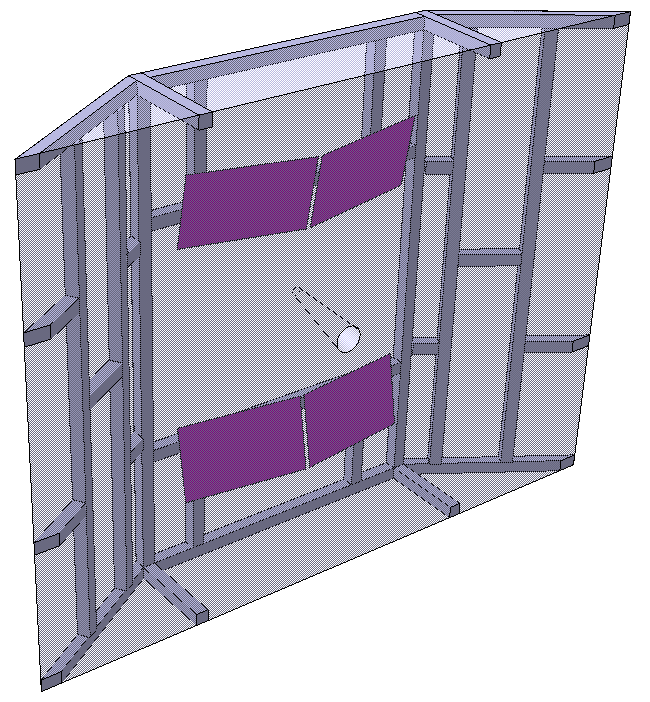
\includegraphics[width=0.6\textwidth]{pictures/PrimitivePhotodetector.png}
\caption{Часть одной из наиболее ранних MC-моделей CBM RICH, в которой фотодетектор был представлен тонкими чувствительными боксами.}
\label{fig:PrimitivePhotodetector}
\end{figure}

% ================================================================================================================
\subsubsection{Модель без магнитного экрана}\label{sec:secNoMagScreen}

Длительное время MC-модель CBM RICH не имела магнитного экрана, см. \figref{fig:MCgeoMirrorsEvolution}(слева). По этой причине не было необходимости создавать дополнительное пространство для выступающей части, что делало форму материнского объёма значительно более простой.

% ================================================================================================================
\subsubsection{Модель с промежуточным объёмом для магнитного экрана}\label{sec:secInterVolMagScreen}

В первой версии MC-модели с магнитным экраном был введён дополнительный промежуточный объём, позиционированный параллельно системе координат объёма радиатора. В него были на одном уровне помещены пластины, представляющие стенки экрана и ещё два контейнера --- с МА~ФЭУ и электроникой (см. \figref{fig:ShieldingBoxMC}). На момент написания работы магнитный экран выполнен как набор пластин, помещённых непосредственно в контейнер для камеры. Принципиальным отличием является то, что поворот и позиционирование экрана теперь выполняется вместе со всей камерой в системе координат объёма радиатора, в то время как в старой модели --- отдельно в системе координат промежуточного контейнера.

% ================================================================================================================
\subsubsection{Модель с зазором между зеркалами}\label{sec:secMirrorsEvolution}

Значительным улучшением в проекте CBM RICH стал переход от формы зеркал, симметричной относительно горизонтальной плоскости, к особой форме, позволяющей стыковать два зеркала практически без зазора (см. \figref{fig:MCgeoMirrorsEvolution}). Изначально рассматривался вариант, в котором одно зеркало выполнено из долей двух типов. Тогда для того, чтобы центр сферической поверхности располагался на расстоянии (над для верхнего зеркала и под --- для нижнего), необходимо было поворачивать каждое зеркало. Новые зеркала не требует поворота, т.к. они имеют форму соответствующего сегмента сферы. Однако это приводит к необходимости иметь не 2, а 4 типоразмера сегментов зеркал и немного усложняет их изготовление (см. \figref{fig:Mirrors4types}).

\begin{figure}[H]
\begin{minipage}[b]{0.495\textwidth}
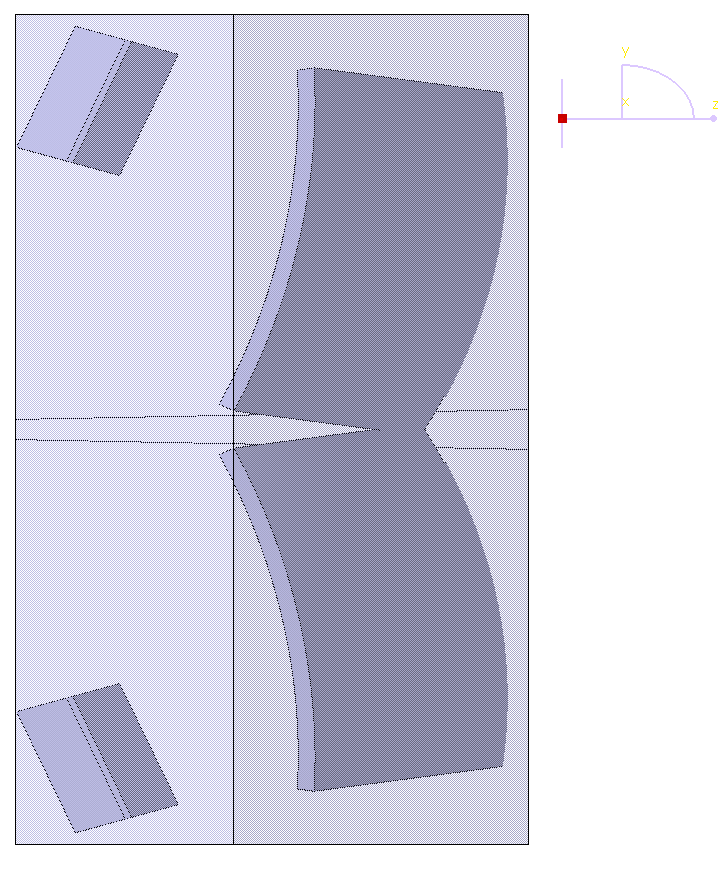
\includegraphics[width=1.0\textwidth]{pictures/RICH_MC_evolution_before.png}
\end{minipage}
\hspace{0.01\textwidth}
\begin{minipage}[b]{0.495\textwidth}
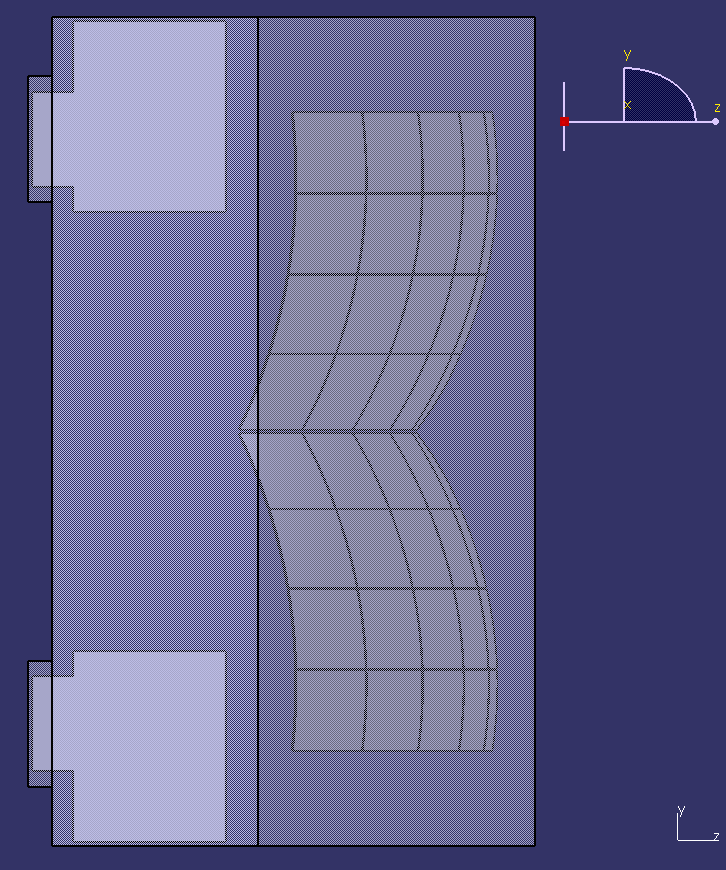
\includegraphics[width=1.0\textwidth]{pictures/RICH_MC_evolution_after.png}
\end{minipage}
\caption{Модель со старыми зеркалами (слева) и модель с новыми зеркалами (справа).}
\label{fig:MCgeoMirrorsEvolution}
\end{figure}

\begin{figure}[H]
\centering
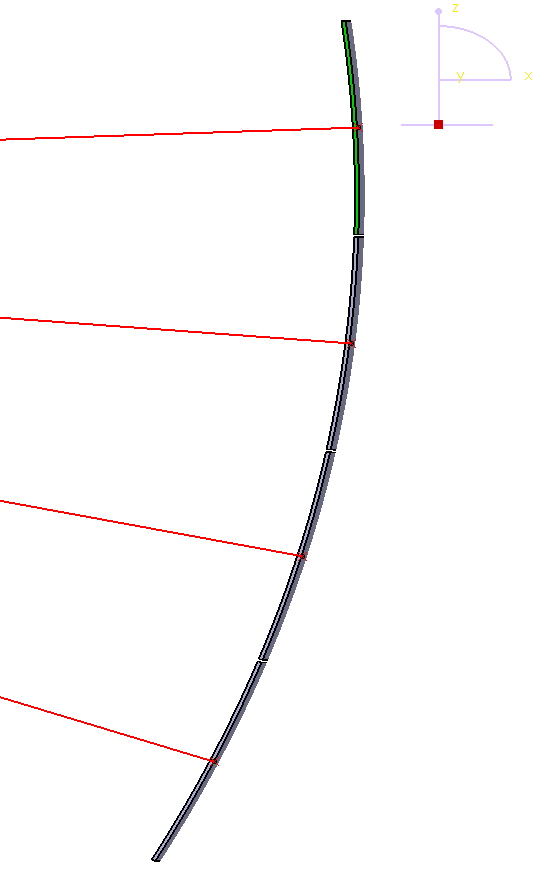
\includegraphics[width=0.3\textwidth]{pictures/Mirrors_4types_of_segments.png}
\caption{4 типоразмера сегментов зеркал, позволяющие собрать фокусирующую систему без зазоров.}
\label{fig:Mirrors4types}
\end{figure}

% ================================================================================================================
\subsubsection{Модель с ``малой рамой''}\label{sec:secModelWithSmallFrame}

На раннем этапе была предложена конструкция опор зеркал, которая в дальнейшем была отвергнута из-за слишком большого количества материала в аксептансе. На \figref{fig:SmallFrameCADandMC} показана модель опор зеркал в САПР (слева) и в CbmRoot (справа).

Особенностью данной модели является то, что она имеет множество опорных балок, хорошо моделирующихся примитивом trap, но имеющих разные размеры.
По мере работы над этой геометрией возникла необходимость подгона полученных от инженеров в САПР форм примитивами trap.
Для этого необходимо было выполнять множесво вспомогателных построений, которые представлялось возможным автоматизировать.
В результате появился \macroname{TrapCreator}, ставший прототипом \macroname{PrimitiveCreator}.

Трапецоиды в данной модели аппроксимируют сложный профиль, имеющий полости. Для сохранения эквивалентного количества материала каждый трапецоид из алюминия имеет дочерний объём из материала радиатора, причём поперечное сечение прямоугольного кольца равно поперечному сечению исходного профиля (см. секцию~\ref{}). Дочерний объём также имеет форму трапецоида, однако его параметры возможно получить тоже только с помощью вспомогательных построений. Для автоматизации расчётов параметров внутреннего трапецоида был разработан документ, называемый hollow_part_template

% \todo
% написать что-то о реализации
% Много трапов, поэтому был разработан hollow trap template и trap-creator, который потом эволюционировал в Primitive_creator

\begin{figure}[H]
\begin{minipage}[b]{0.495\textwidth}
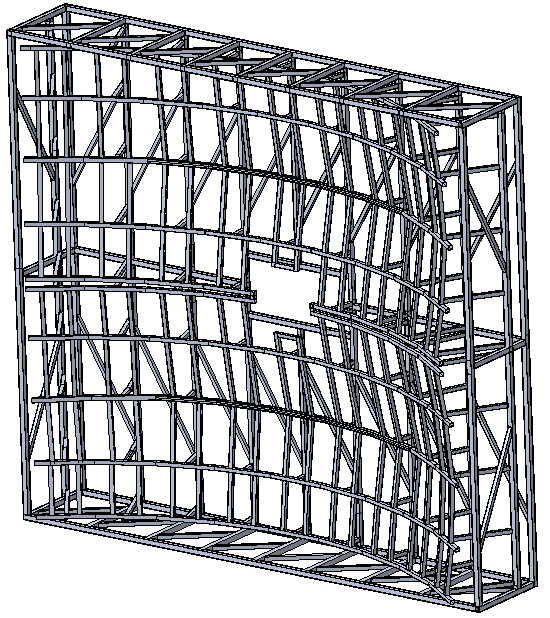
\includegraphics[width=1.0\textwidth]{pictures/Frame_small_CAD.png}
\end{minipage}
\hspace{0.01\textwidth}
\begin{minipage}[b]{0.495\textwidth}
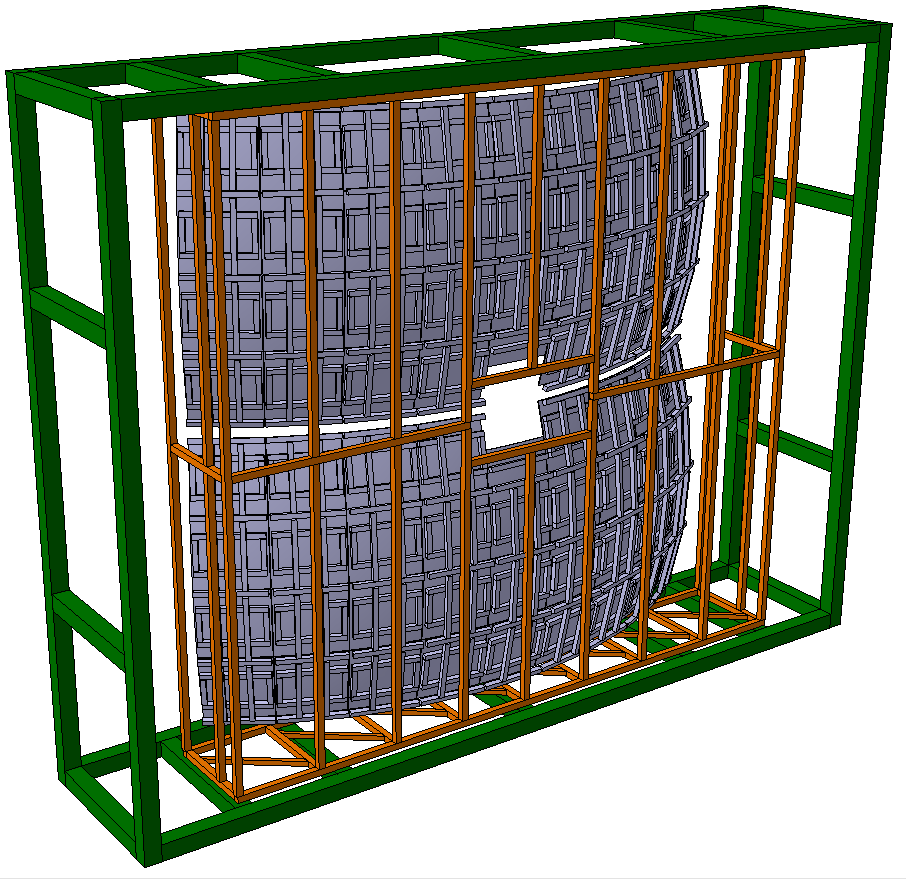
\includegraphics[width=1.0\textwidth]{pictures/Frame_small_MC2.png}
\end{minipage}
\caption{Ранняя модель опор зеркал в САПР CATIA~V5 (слева) и в CbmRoot (справа).}
\label{fig:SmallFrameCADandMC}
\end{figure}

% ================================================================================================================
\subsubsection{Модель с репликой долей зеркал}\label{sec:secModelWithReplMirrors}

% \todo
% Где какие оси, что вокруг чего крутится, реплицируется, ось одна перпенд. другой и т.д.
Примитив cегмент шара (sphere) в наиболее общем виде имеет 6~граней --- внешнюю и внутреннюю сферические поверхности, две плоскости (проходящие через ось Z примитива) и две конические поверхности (имеющие вершины в начале системы координат примитива).
% На самом деле ROOT допускает деление шара как вдоль фи, так и вдоль R и тэта, но в билдере мы реализуем только такое деление, которое приводит к одинаковым формам долек, т.е. только фи.
Для этого примитива допускается реплика только в направлении $\phi$, т.е. сегмент шара разрезается плоскостями, проходящими через ось Z примитива. В результате такого деления сегмент шара разбивается на более мелкие сегменты, стыкующиеся по плоскостям.

Дальнейшее объяснение удобно вести в системе координат примитива sphere и предполагать, что ось Z --- это вертикальная ось.

Контейнер для одной вертикальной полосы
\textit{RICH\textunderscore miror\textunderscore and\textunderscore support\textunderscore belt\textunderscore strip}
имеет форму сегмента шара.
Сборка опорной структуры для одного сегмента зеркала, выполненная с помощью assembly-volume \textit{sup\textunderscore element}, многократно вставляется в
\textit{RICH\textunderscore miror\textunderscore and\textunderscore support\textunderscore belt\textunderscore strip}
с помощью кругового массива вокруг горизонтальной оси, перпендикулярной вертикальной плоскости симметрии сегмента шара контейнера. Здесь возможны варианты, но если задать форму контейнера так, чтобы плоскость симметрии проходила через ось~X (это будет означать, что параметр примитива $\phi_{start} = -\Delta_{\phi}/2$), т.е. совпадала с плоскостью ZX в системе координат примитива, то осью массива будет ось~Y.

Можно также отметить, что 4 различные формы сегментов зеркал, являющиеся дочерними объёмами в контейнере на одном уровне с массивом опорных структур, имеют центр в начале координат сферы контейнера и стыкуются по коническим поверхностям (возможно с зазором).

Для получения одного зеркала выполняется реплицирование контейнера вокруг оси Z (т.е. вдоль направления $\phi$) внутри 
\textit{RICH\textunderscore mirror\textunderscore replica}. 
Последним этапом необходимо поместить всё зеркало в объём газа-радиатора, причём ось~Z в этой системе --- горизонтальная ось пучка. Для этого при позиционировании наобходимо выполнить два последовательных поворота на~\SI{90}{\degree} --- вокруг оси~Z и затем вокруг оси~X --- так, чтобы ось~Z примитива совпадала с осью~Y глобальной системы координат, а ось~X примитива --- с осью~Z глобальной системы координат. % \todo проверить

\begin{figure}[H]
\begin{minipage}[t]{0.495\textwidth}
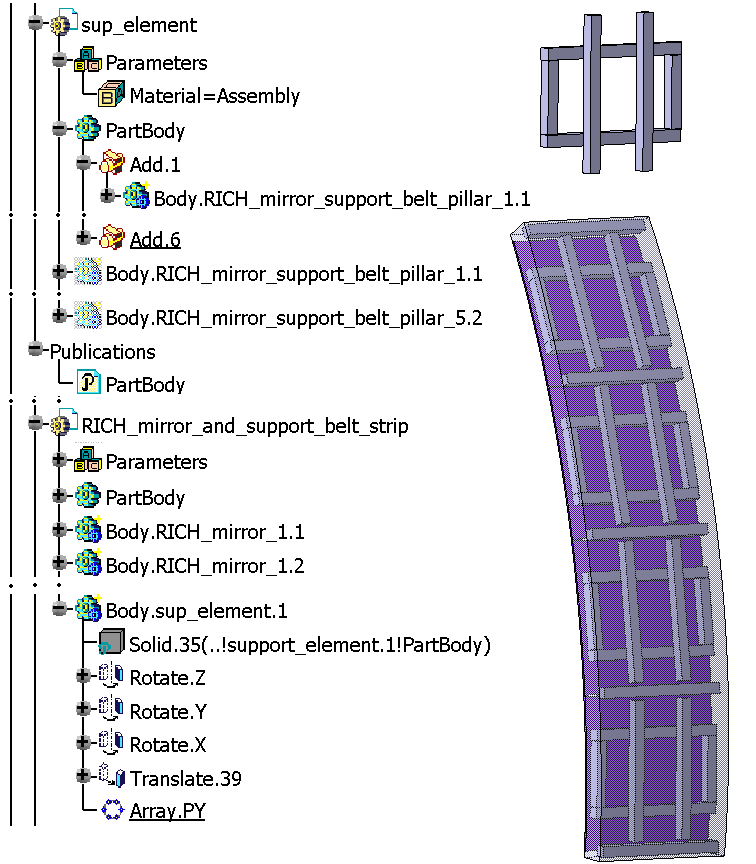
\includegraphics[width=0.95\textwidth]{pictures/CbmRichMirror1.png}
\end{minipage}
\hspace{0.01\textwidth}
\begin{minipage}[t]{0.495\textwidth}
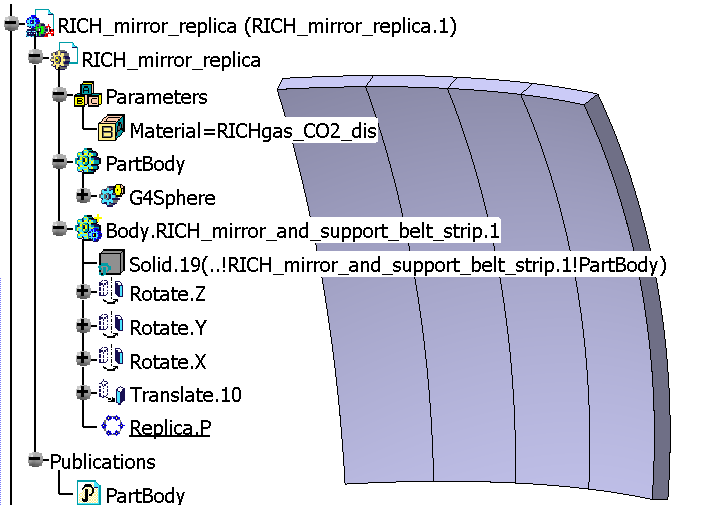
\includegraphics[width=0.95\textwidth]{pictures/CbmRichMirror2.png}
\end{minipage}
\caption{Слева --- контейнер с вставленными в него сегментами зеркал и массивом опор; справа --- реплика из 4-х контейнеров, составляющая часть зеркала.}
\label{fig:ReplicaMirror}
\end{figure}

Данная версия геометрии длительное время использовалась в качестве основной, однако когда возникла необходимость моделировать индивидуальные отклонения сегментов зеркал пришлось от неё отказаться и выполнять независимые вставки отдельных сегментов зеркал с возможностью их независимого позиционирования. % \todo ссылка \ref{}
